\documentclass[]{elsarticle} %review=doublespace preprint=single 5p=2 column
%%% Begin My package additions %%%%%%%%%%%%%%%%%%%
\usepackage[hyphens]{url}



\usepackage{lineno} % add
\providecommand{\tightlist}{%
  \setlength{\itemsep}{0pt}\setlength{\parskip}{0pt}}

\usepackage{graphicx}
\usepackage{booktabs} % book-quality tables
%%%%%%%%%%%%%%%% end my additions to header

\usepackage[T1]{fontenc}
\usepackage{lmodern}
\usepackage{amssymb,amsmath}
\usepackage{ifxetex,ifluatex}
\usepackage{fixltx2e} % provides \textsubscript
% use upquote if available, for straight quotes in verbatim environments
\IfFileExists{upquote.sty}{\usepackage{upquote}}{}
\ifnum 0\ifxetex 1\fi\ifluatex 1\fi=0 % if pdftex
  \usepackage[utf8]{inputenc}
\else % if luatex or xelatex
  \usepackage{fontspec}
  \ifxetex
    \usepackage{xltxtra,xunicode}
  \fi
  \defaultfontfeatures{Mapping=tex-text,Scale=MatchLowercase}
  \newcommand{\euro}{€}
\fi
% use microtype if available
\IfFileExists{microtype.sty}{\usepackage{microtype}}{}
\usepackage[left=3cm,right=3cm,top=3cm,bottom=3cm]{geometry}
\bibliographystyle{elsarticle-harv}
\usepackage{longtable}
\ifxetex
  \usepackage[setpagesize=false, % page size defined by xetex
              unicode=false, % unicode breaks when used with xetex
              xetex]{hyperref}
\else
  \usepackage[unicode=true]{hyperref}
\fi
\hypersetup{breaklinks=true,
            bookmarks=true,
            pdfauthor={},
            pdftitle={Living on the edge: crop boundary effects on canola and wheat yields in Alberta},
            colorlinks=false,
            urlcolor=blue,
            linkcolor=magenta,
            pdfborder={0 0 0}}
\urlstyle{same}  % don't use monospace font for urls

\setcounter{secnumdepth}{5}
% Pandoc toggle for numbering sections (defaults to be off)

% Pandoc citation processing
\newlength{\csllabelwidth}
\setlength{\csllabelwidth}{3em}
\newlength{\cslhangindent}
\setlength{\cslhangindent}{1.5em}
% for Pandoc 2.8 to 2.10.1
\newenvironment{cslreferences}%
  {}%
  {\par}
% For Pandoc 2.11+
\newenvironment{CSLReferences}[3] % #1 hanging-ident, #2 entry spacing
 {% don't indent paragraphs
  \setlength{\parindent}{0pt}
  % turn on hanging indent if param 1 is 1
  \ifodd #1 \everypar{\setlength{\hangindent}{\cslhangindent}}\ignorespaces\fi
  % set entry spacing
  \ifnum #2 > 0
  \setlength{\parskip}{#2\baselineskip}
  \fi
 }%
 {}
\usepackage{calc} % for calculating minipage widths
\newcommand{\CSLBlock}[1]{#1\hfill\break}
\newcommand{\CSLLeftMargin}[1]{\parbox[t]{\csllabelwidth}{#1}}
\newcommand{\CSLRightInline}[1]{\parbox[t]{\linewidth - \csllabelwidth}{#1}}
\newcommand{\CSLIndent}[1]{\hspace{\cslhangindent}#1}

% Pandoc header
\makeatletter \def\ps@pprintTitle{  \let\@oddhead\@empty  \let\@evenhead\@empty  \def\@oddfoot{\centerline{\thepage}} \let\@evenfoot\@oddfoot} \makeatother \usepackage{float} \floatplacement{figure}{H} \newcommand{\beginsupplement}{\setcounter{table}{0} \renewcommand{\thetable}{S\arabic{table}} \setcounter{figure}{0} \renewcommand{\thefigure}{S\arabic{figure}}} \usepackage{setspace} \linenumbers
\usepackage{booktabs}
\usepackage{longtable}
\usepackage{array}
\usepackage{multirow}
\usepackage{wrapfig}
\usepackage{float}
\usepackage{colortbl}
\usepackage{pdflscape}
\usepackage{tabu}
\usepackage{threeparttable}
\usepackage{threeparttablex}
\usepackage[normalem]{ulem}
\usepackage{makecell}
\usepackage{xcolor}



\begin{document}
\begin{frontmatter}

  \title{Living on the edge: crop boundary effects on canola and wheat yields in Alberta}
    \author[University of Calgary]{Samuel V. J. Robinson\corref{1}}
   \ead{samuel.robinson@ucalgary.ca} 
    \author[University of Calgary]{Lan H. Nguyen}
   \ead{hoanglan.nguyen@ucalgary.ca} 
    \author[University of Calgary]{Paul Galpern}
   \ead{paul.galpern@ucalgary.ca} 
      \address[University of Calgary]{2500 University Drive NW, Calgary, AB}
      \cortext[1]{Corresponding Author}
  
  \begin{abstract}
  Abstract goes here
  \end{abstract}
   \begin{keyword} beetles; spiders; harvestmen;\end{keyword}
 \end{frontmatter}

\newpage
\doublespacing

\hypertarget{introduction}{%
\section{Introduction}\label{introduction}}

Intensive agricultural production has increased over the last 100 years, and agricultural land now makes up over a third of ice-free land on Earth
This has allowed increases in human population and increased (global) stability in production
However, this is not without cost, as higher-diversity non-crops are converted to lower-diversity crops, resulting in loss of habitat and overall biodiversity of non-target organisms
Maintaining both biodiversity and production in agroecosystems represents a seldom-considered goal of conservationists and agronomists, and hold the potential for win-win scenarios
Key to this is the preservation of semi-natural land (SNL), which represents the interface between crops and non-crops within agroecosystems

SNL in and around crops is important for both agricultural production and conservation
They are habitat for mobile organisms, and can therefore act as sources of ecosystem services such as pollination or pest control (Albrecht \emph{et al.} (2020); Gardner \emph{et al.} (2021))
They also can create microclimate effects that reduce extreme temperature, trap moisture, and reduce wind speed (Kort (1988))
Unfortunately, most of the research is concentrated in Europe, and they tend to be less-studied on other continents
In particular, North American agroecosystems have larger fields, different crop varieties, and agronomic practices, all of which could negate or confound potential effects of SNL

SNL may affect yields at intermediate distances, depending on the spatial scale at which ecosystem services operate
Edge effects cause low yields at the edge of crops because of sparse or late seedling emergence, poor microclimate, and competition with weeds
At the same time, the centre of large fields will not receive ecosystem services if they decay with distance from edges (Kowalchuk \& Jong (1995))
For example, pollination services from central place foragers that nest in SNL but forage in crops drops rapidly with distance
Therefore, yield may be maximized at intermediate distances, where the ecosystem services cancel out negative edge effects (e.g. Van Vooren \emph{et al.} (2017))
This suggests a ``goldilocks" field size, where negative edge effects are canceled out by ecosystem services

Studies of SNL effects on crop yield also suffer from limited scope (e.g.~few crop types) and small sample sizes, limiting inference and reducing generality (but see wheat study)
Meta-analyses have been the standard solution to this problem, but precision yield data holds enormous promise.
However, its use is limited for several reasons: 1) Lack of standardized formats between equipment types, 2) Sensor calibration required for field-level accuracy, and 3) unfamiliarity with spatial statistics.
Ecosystem services can influence both the mean and variability of yield in agroecosystems (Redhead \emph{et al.} (2020)).
Typically only averages (means) are considered, but higher stability (lower variance) in yield can also be valuable.
There are few studies of yield variability (only those with large datasets), but precision yield data opens up the possibility of modeling within-field variability, as well as average yield.

In this paper we ask:
1. How does crop yield change with distance from the edge of field?
2. Does this depend on type of field edge?
3. Is there an intermediate distance where yield is maximized or variance is minimized?

\hypertarget{methods}{%
\section{Methods}\label{methods}}

\hypertarget{data-collection}{%
\subsection{Data collection}\label{data-collection}}

Precision yield data were collected directly from farmers across Alberta.
Farmers were solicited for yield data through local agronomists, and we received 298 field-years of data from 5 growers across a total of 7 years (2014-2020).
We converted raw data to a standard csv format using Ag Leader SMS.
72\% of the crop types where either wheat (\emph{Triticum aestivum}) or canola (\emph{Brassica napus}), two of the most common crops in rotation in Alberta.
The remaining crop types had low replication, so we constrained our analysis to only field-years containing wheat (94) or canola (119).
Individual fields contained between 1 to 5 years of data (mean: 2.7), containing a total of 18.4 million data points.

Yield data is collected in rectangles of the same length as the data interval (distance = combine ground speed \(\times\) interval, typically 1 second) and the same width as the combine header (5-7 m, adjusted to account for overlap with adjacent swaths).
We extracted the size of each polygon (m\(^2\)), dry yield (tonnes), and the spatial location, and the sequence of collection (1 - end of harvest)
Because of the large number of yield rectangles per field (30-800 thousand), we used the centroid of each polygon as its location, treating areal data as point data
Seeding and application rates were constant across fields, so we did not consider inputs in our analysis
We used dry yield (tonnes of seed/hectare minus recorded crop moisture) as our measure of crop yield
Precision yield data can be highly variable and is prone to extreme outliers (both positive and negative), especially when combine ground speeds are low and at the beginning of rows
Therefore, we filtered data that lay outside the 95th percentiles of yield within each field, values less than or equal to zero, and values outside of the 95th percentiles of ground speed.
Due to the large number of data at each field, we sub-sampled to 50,000 data points per field to reduce computation time.

Field boundaries were automatically digitized using buffers from the yield data locations, then manually checked using satellite imagery from Google Earth and classified land cover data from AAFC.
Crop boundaries are flexible, and often change yearly depending on planting and emergence conditions (e.g.~flooding during some years).
Ephemeral wetlands are flooded during some years, but consist mainly of grasses during dry years, and grass boundaries can change if fields are used for as haying or pasture during crop rotation.
This makes accurate and consistent classification of field boundaries difficult.
We defined the following general categories for field boundaries:
1. Standard: grassy field edge, staging yard, or road right-of-way (grassy strip typically 5-10m wide)
2. Wetland: permanent wetland; borders are largely unchanged from year-to-year
3. Shelterbelt: permanent windbreaks, shelterbelts, remnant forests, or shrublands
4. Other crop: annual crop or pasture with little or no visible boundary between planted areas
5. Bare: unplanted, fallow, flooded area, temporary wetland (only present for a single season), staging yard, oil and gas equipment, or road without a planted boundary
6. Grassland: permanent seminatural grassland or pasture (not in rotation)

\begin{verbatim}
<!-- STANDARD -->
<!-- WETLAND -->
<!-- SHELTERBELT -->
<!-- OTHERCROP -->
<!-- BARE -->
<!-- GRASSLAND -->
\end{verbatim}

\hypertarget{analysis}{%
\subsection{Analysis}\label{analysis}}

Yield data from each field contains both random and systematic errors that must be modeled in order to reveal underlying changes in yield.
We fit an additive model of the effect of boundary distance on crop yield while accounting for within-field spatial variation and temporal variation in the data.
Crop yield can vary within a field due to soil conditions, moisture, seeding rates, herbicide application, and previous agricultural practices.
Ground speed is extremely important to yield monitor accuracy (Arslan \& Colvin 2002), with low ground speed registering higher yields.
Sensor calibration can reduce combine-level bias (such as a combine recording consistently higher/lower yields across fields), this does not address sensor drift that occurs over time.
This may be caused by sensors accumulating debris during harvest (especially in canola, pers. comm. Trent Clark), leading to changes in accuracy and bias over time.
To model this, we fit the following model to each field-year of data:

\begin{equation}
  \begin{split}
  \sqrt{yield} \sim & Normal (\mu, \sigma)\\
  \mu = & Intercept + log(\text{Polygon Size}) + f(\text{Edge Distance}, b=12)_i + \\
   & f(\text{Easting}, \text{Northing}, b=60) + f(\text{Sequence}, b=60) \\
  log(\sigma) =  & Intercept + log(\text{Polygon Size}) + f(\text{Edge Distance}, b=12)_i + \\
   & f(\text{Easting}, \text{Northing}, b=60) + f(\text{Sequence}, b=60) \\
  \end{split}
  \end{equation}

\begin{itemize}
\tightlist
\item
  where:
\end{itemize}

\begin{enumerate}
\def\labelenumi{\arabic{enumi}.}
\tightlist
\item
  Polygon Size = distance traveled \(\times\) width of header bar (\(m^2\))
\item
  Edge Distance = distance from field edge type \emph{i} (m)
\item
  Easting, Northing = distance from centre of field (m)
\item
  Sequence = order of harvest within field (1--N points)
\item
  f(x,b) = penalized thin-plate regression spline, where \emph{x} is the predictor and \emph{b} is the number of basis dimensions
\end{enumerate}

In addition to modeling edge effects (our variable of interest), this model also accounts for a) differences in combine speed, b) within-field spatial variation not related to edges, and d) shifts in combine accuracy during harvest.
Spatial or temporal variation can be modelled using a Gaussian Process Model (e.g.~Kriging, SPDE Approximations) but this was computationally unfeasible with 50,000 data points per field.
Penalized splines offer a compromise, as they account for nonlinear ``wiggly" relationships in the same way as Gaussian processes but using a reduced number of dimensions and computation time.
The number of basis dimensions was checked with the \emph{gam.check} function from \emph{mgcv}.
The relationship between polygon size (i.e.~ground speed) and yield was modeled with a log-linear relationship with a single slope term, as this closely matched smoothed versions.
All models were fit in \emph{R} using the \emph{mgcv} library (version 1.8.36, Wood 2017), and figures were created with \emph{ggplot2} and \emph{ggpubr} (versions 3.3.3, Wickham 2016; and 0.4.0, Kassambara 2020).

Despite the use of spatial and temporal smoothers, the residuals in most of the models displayed a large amount of spatial and temporal autocorrelation.
\emph{Not really sure how we can get around this. In practice, this means that SEs for all coefficients are too small (i.e.~we gathered 1000 points, but because they're spatially related, it's only equivalent to 100 points).}

To consider results from all field-level models together, we fit models independent of each other and fit an ``overall'' smoother as averages of the field-level smoothers.
However, this does not account for uncertainty in the field-level smoothers, so we used an approach similar to bootstrapping of hierarchical mixed effects models:
1. Extract single posterior sample (\emph{rnorm} in R) of smoother parameters from each field-level model using coefficient estimates and standard error
2. Use posterior sample to create a new smoother from each field
3. Fit new model of new smoothers from all fields, and save this ``meta-smoother''
4. Repeat 1000 times, and calculate coverage intervals (5-95\% percentiles) on saved meta-smoothers
This gives coverage intervals (CIs) for the ``average'' smoother while accounting for field-level variability, and is conceptually similar to a meta-analysis.

\hypertarget{results}{%
\section{Results}\label{results}}

\hypertarget{field-boundaries}{%
\subsection{Field boundaries}\label{field-boundaries}}

``Standard'' (grassy border) was the most common boundary type, followed by ``Shelterbelt'' and ``Other Crop'' (Table \ref{tab:boundaryTypes}).

\begin{table}

\caption{\label{tab:boundaryTypes}Mean and SD of proportion of boundary types across all fields, along with the number of fields bordered by at least some of the boundary type.}
\centering
\begin{tabular}[t]{l|r|r|r}
\hline
Type & Mean & SD & Number of Fields\\
\hline
Bare & 0.0419 & 0.0618 & 126\\
\hline
Grassland & 0.0506 & 0.1254 & 84\\
\hline
Other Crop & 0.1515 & 0.2187 & 143\\
\hline
Shelterbelt & 0.3180 & 0.2236 & 274\\
\hline
Standard & 0.3870 & 0.2041 & 283\\
\hline
Wetland & 0.0509 & 0.0836 & 120\\
\hline
\end{tabular}
\end{table}

\hypertarget{canola}{%
\subsection{Canola}\label{canola}}

Average canola yield tended to increase with distance from Standard and Other Crop boundaries, leveling off at about 25 m (Figure \ref{fig:canolaPlot} top row, Other crop and Standard panels); yield was approximately 0.1 T/ha (1.5 bu/ac) lower at the edge for both of these boundary types.
Interestingly, Shelterbelts were well-represented in the data (Table \ref{tab:boundaryTypes}) but the negative edge effect was not strong (Figure \ref{fig:canolaPlot} top row, Shelterbelt panel), indicating that they may provide better micro-climates for crops located near them.
Other boundary types were less common in the data and had correspondingly weaker effects on mean yield, but all showed a small negative edge effect.

Yield variability (SD of yield) also varied with distance from the edge of the field, but this

\begin{figure}
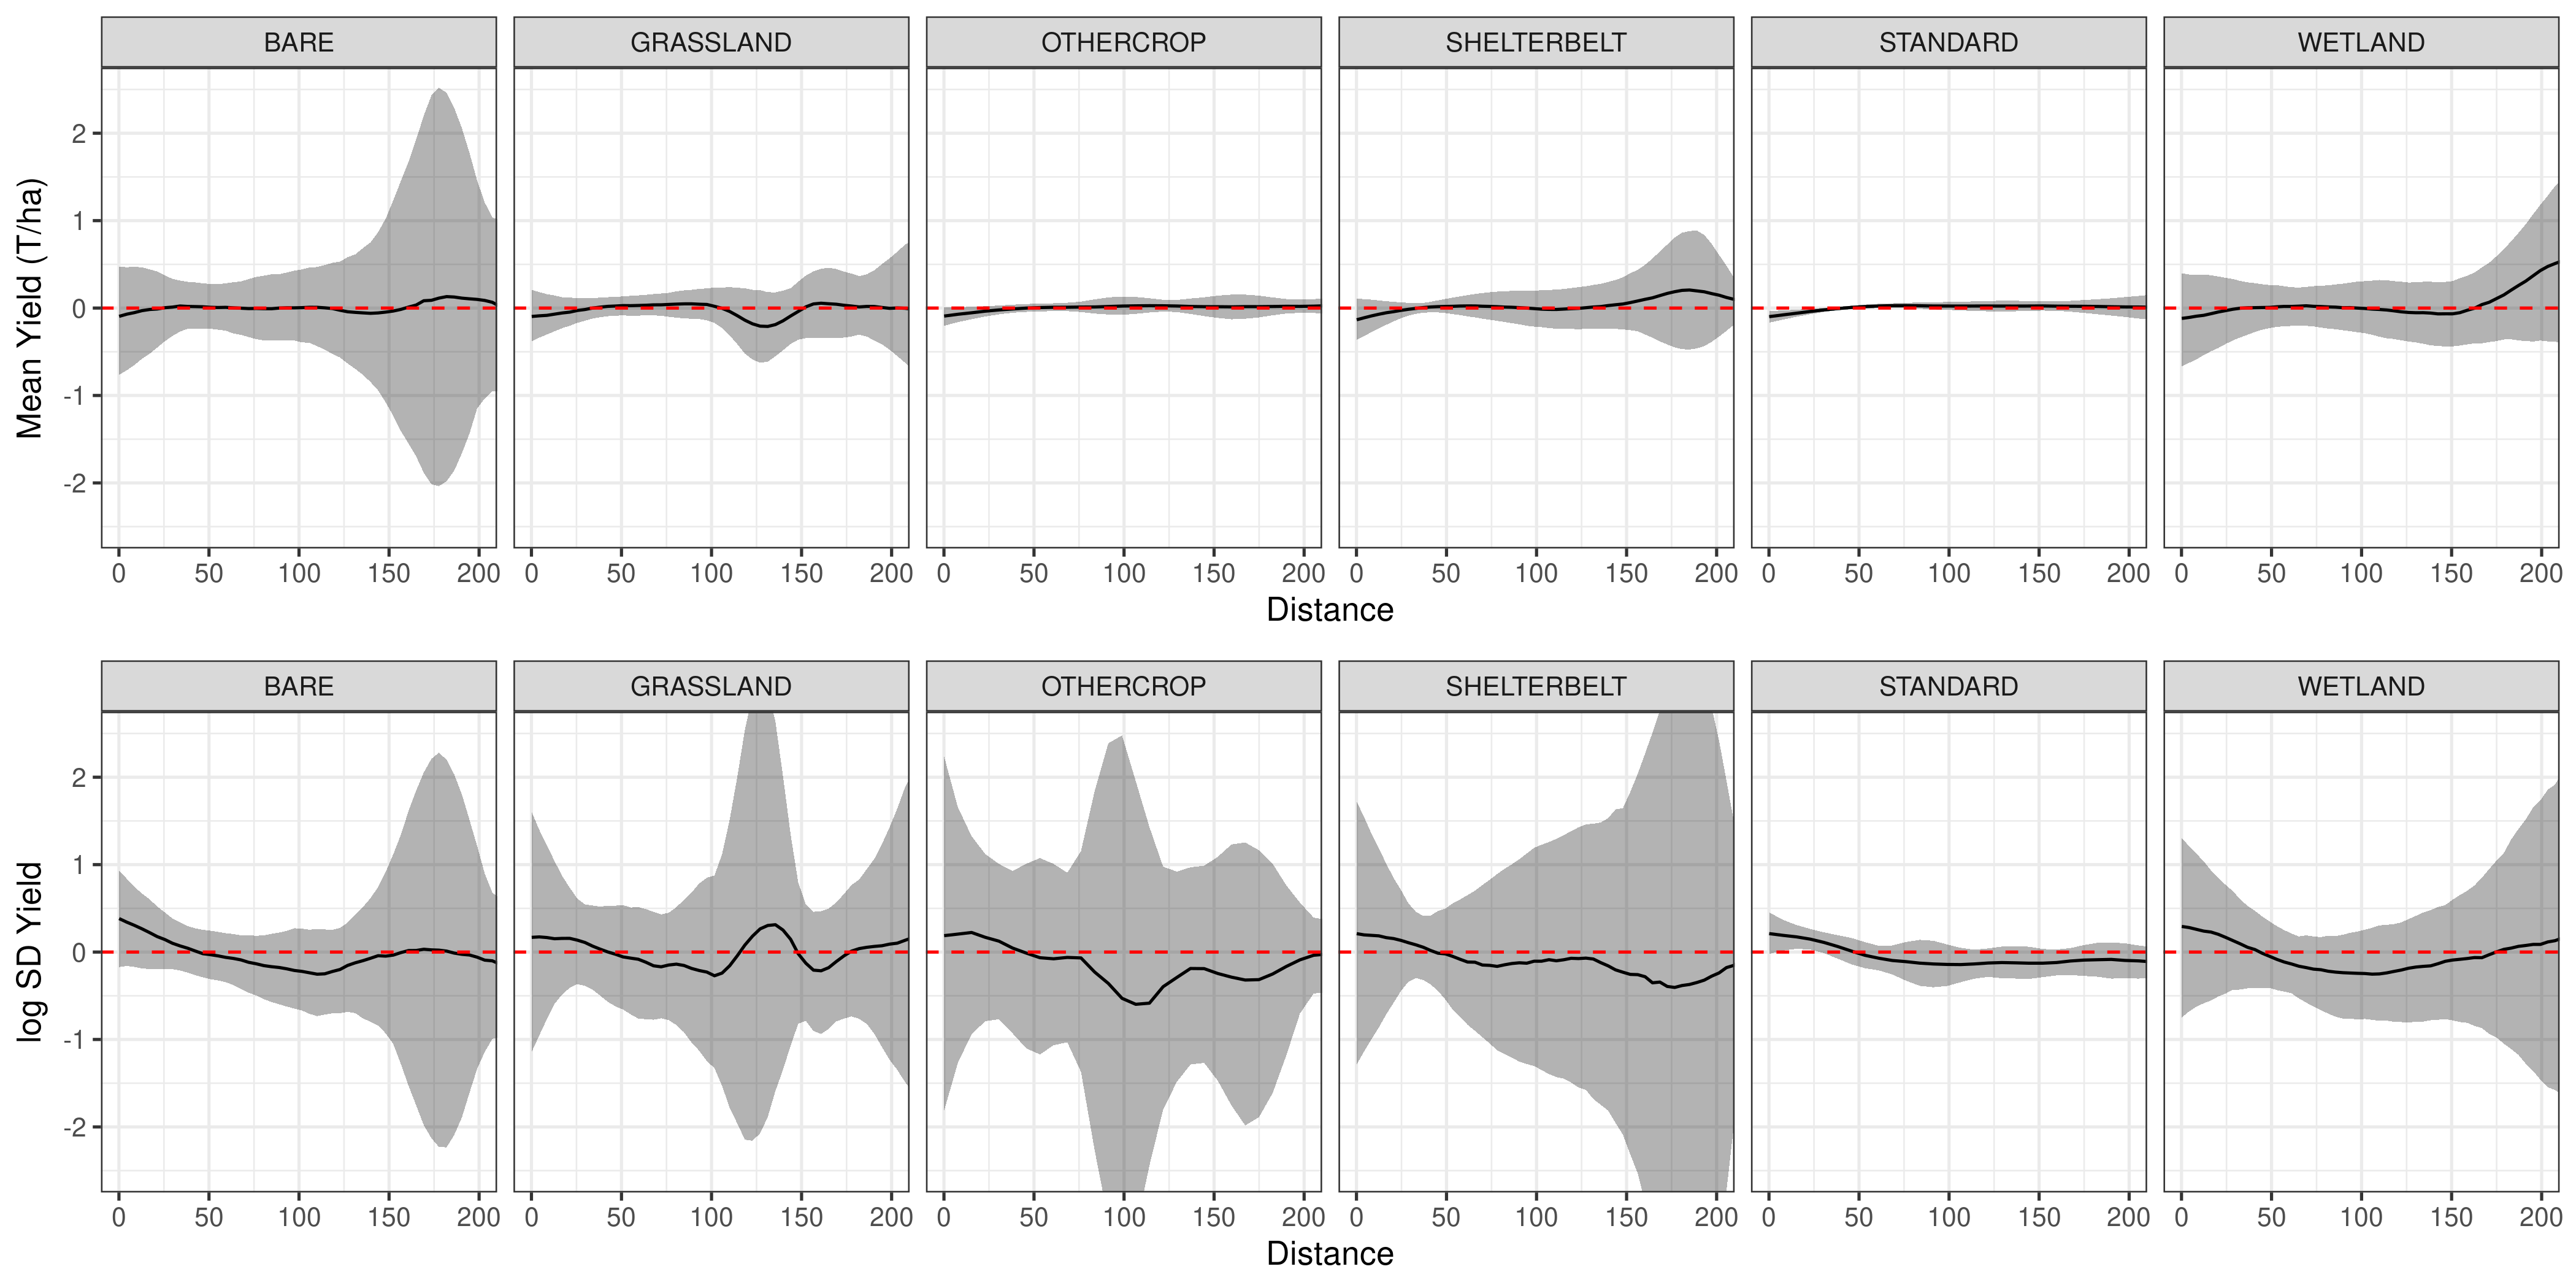
\includegraphics[width=1\linewidth]{../Figures/ModelSummary3a_canola} \caption{Field boundary effect on canola yield, accounting for the effect of combine speed, spatial variation, and harvest sequence. Upper panel represents mean yield, while the lower panel represents yield variation (i.e. "patchiness").}\label{fig:canolaPlot}
\end{figure}

\hypertarget{wheat}{%
\subsection{Wheat}\label{wheat}}

Average wheat yield (Figure \ref{fig:wheatPlot}

\begin{figure}
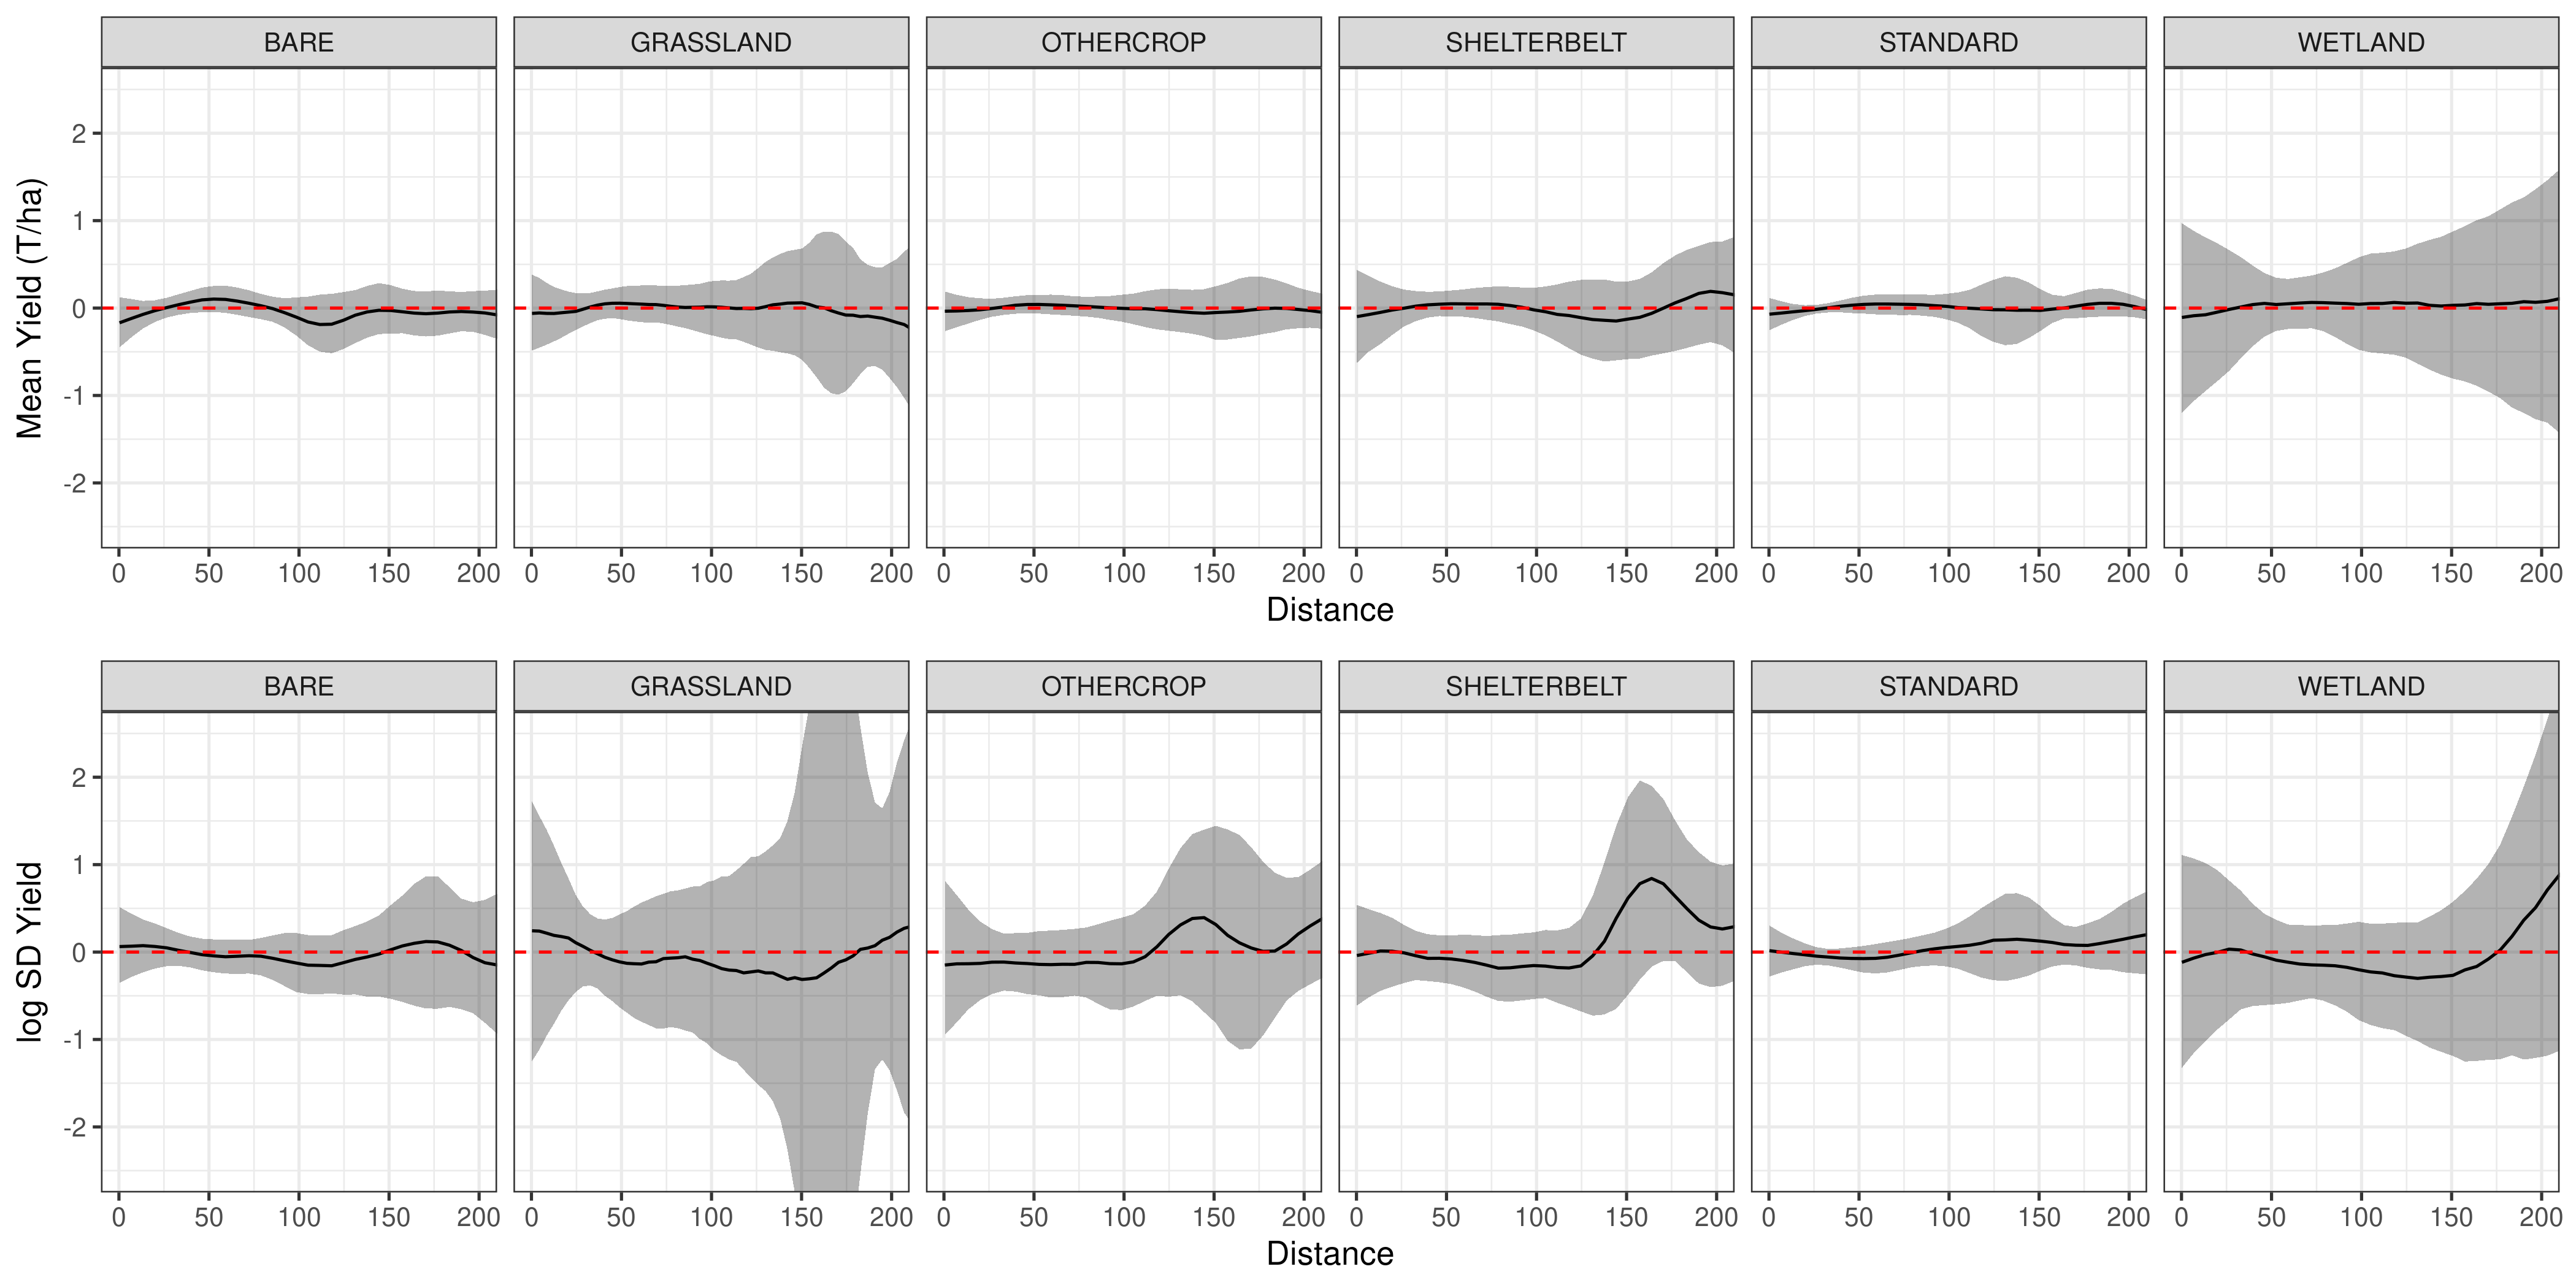
\includegraphics[width=1\linewidth]{../Figures/ModelSummary3a_wheat} \caption{Field boundary effect on canola yield, accounting for the effect of combine speed, spatial variation, and harvest sequence. Upper panel represents mean yield, while the lower panel represents yield variation (i.e. "patchiness").}\label{fig:wheatPlot}
\end{figure}

\hypertarget{discussion}{%
\section{Discussion}\label{discussion}}

Discussion here

\hypertarget{author-contributions}{%
\section{Author Contributions}\label{author-contributions}}

SVJR and PG conceived of the project.
SVJR collected data, conducted analysis, and wrote the manuscript.

\hypertarget{acknowledgements}{%
\section{Acknowledgements}\label{acknowledgements}}

We thank Trent Clark, Dean Hubbard, Alvin French, and Kristina Polziehn for providing yield data for us, and providing insight on their yield data.
We also thank Autumn Barnes and Keith Gabert of the Canola Council of Canada, and Laurel Thompson and JP Pettyjohn of Lakeland College for connecting us with farmers and agronomists.
Funding for this research was provided by Ducks Unlimited Canada's Institute for Wetland and Waterfowl Research, the Alberta Canola Producers Commission, Manitoba Canola Growers Association, SaskCanola, the Alberta Biodiversity Monitoring Institute, and the Alberta Conservation Association.

\hypertarget{references}{%
\section*{References}\label{references}}
\addcontentsline{toc}{section}{References}

\hypertarget{refs}{}
\begin{CSLReferences}{1}{0}
\leavevmode\hypertarget{ref-albrecht2020}{}%
Albrecht, M., Kleijn, D., Williams, N.M., Tschumi, M., Blaauw, B.R., Bommarco, R., \emph{et al.} (2020). The effectiveness of flower strips and hedgerows on pest control, pollination services and crop yield: A quantitative synthesis. \emph{Ecology Letters}.

\leavevmode\hypertarget{ref-arslan2002}{}%
Arslan, S. \& Colvin, T.S. (2002). An evaluation of the response of yield monitors and combines to varying yields. \emph{Precision Agriculture}, 3, 107--122.

\leavevmode\hypertarget{ref-gardner2021}{}%
Gardner, E., Breeze, T.D., Clough, Y., Smith, H.G., Baldock, K.C.R., Campbell, A., \emph{et al.} (2021). Field boundary features can stabilise bee populations and the pollination of mass-flowering crops in rotational systems. \emph{Journal of Applied Ecology}, In press.

\leavevmode\hypertarget{ref-kassambara2020}{}%
Kassambara, A. (2020). \emph{{ggpubr}: 'ggplot2' based publication ready plots}.

\leavevmode\hypertarget{ref-kort1988}{}%
Kort, J. (1988). 9. Benefits of windbreaks to field and forage crops. \emph{Agriculture, Ecosystems {\&} Environment}, 22-23, 165--190.

\leavevmode\hypertarget{ref-kowalchuk1995}{}%
Kowalchuk, T.E. \& Jong, E. de. (1995). Shelterbelts and their effect on crop yield. \emph{Canadian Journal of Soil Science}, 75, 543--550.

\leavevmode\hypertarget{ref-redhead2020}{}%
Redhead, J.W., Oliver, T.H., Woodcock, B.A. \& Pywell, R.F. (2020). The influence of landscape composition and configuration on crop yield resilience. \emph{Journal of Applied Ecology}.

\leavevmode\hypertarget{ref-vanVooren2017}{}%
Van Vooren, L., Bert, R., Steven, B., Pieter, D.F., Victoria, N., Paul, P., \emph{et al.} (2017). Ecosystem service delivery of agri-environment measures: A synthesis for hedgerows and grass strips on arable land. \emph{Agriculture, Ecosystems {\&} Environment}, 244, 32--51.

\leavevmode\hypertarget{ref-wickham2016}{}%
Wickham, H. (2016). \emph{{ggplot2}: Elegant graphics for data analysis}. Springer-Verlag New York.

\leavevmode\hypertarget{ref-wood2017}{}%
Wood, S.N. (2017). \emph{Generalized additive models: An introduction with {R}}. CRC press.

\end{CSLReferences}

\newpage

\hypertarget{appendix-a-supplementary-material}{%
\section*{Appendix A: Supplementary Material}\label{appendix-a-supplementary-material}}
\addcontentsline{toc}{section}{Appendix A: Supplementary Material}

\begin{figure}
\includegraphics[width=1\linewidth]{../Figures/ModelSummary3b_canola} \caption{Effect of polygon area and harvest sequence on canola yield. Polygon area is equivalent to ground }\label{fig:unnamed-chunk-2}
\end{figure}

\begin{figure}
\includegraphics[width=1\linewidth]{../Figures/ModelSummary3b_wheat} \caption{Temp}\label{fig:unnamed-chunk-3}
\end{figure}


\end{document}

